% $Id: template.tex 11 2007-04-03 22:25:53Z jpeltier $

\documentclass{vgtc}                          % final (conference style)
%\documentclass[review]{vgtc}                 % review
%\documentclass[widereview]{vgtc}             % wide-spaced review
%\documentclass[preprint]{vgtc}               % preprint
%\documentclass[electronic]{vgtc}             % electronic version


%% Uncomment one of the lines above depending on where your paper is
%% in the conference process. ``review'' and ``widereview'' are for review
%% submission, ``preprint'' is for pre-publication, and the final version
%% doesn't use a specific qualifier. Further, ``electronic'' includes
%% hyperreferences for more convenient online viewing.

%% Please use one of the ``review'' options in combination with the
%% assigned online id (see below) ONLY if your paper uses a double blind
%% review process. Some conferences, like IEEE Vis and InfoVis, have NOT
%% in the past.

%% Figures should be in CMYK or Grey scale format, otherwise, colour 
%% shifting may occur during the printing process.

%% These few lines make a distinction between latex and pdflatex calls and they
%% bring in essential packages for graphics and font handling.
%% Note that due to the \DeclareGraphicsExtensions{} call it is no longer necessary
%% to provide the the path and extension of a graphics file:
%% \includegraphics{diamondrule} is completely sufficient.
%%
\ifpdf%                                % if we use pdflatex
  \pdfoutput=1\relax                   % create PDFs from pdfLaTeX
  \pdfcompresslevel=9                  % PDF Compression
  \pdfoptionpdfminorversion=7          % create PDF 1.7
  \ExecuteOptions{pdftex}
  \usepackage{graphicx}                % allow us to embed graphics files
  \DeclareGraphicsExtensions{.pdf,.png,.jpg,.jpeg} % for pdflatex we expect .pdf, .png, or .jpg files
\else%                                 % else we use pure latex
  \ExecuteOptions{dvips}
  \usepackage{graphicx}                % allow us to embed graphics files
  \DeclareGraphicsExtensions{.eps}     % for pure latex we expect eps files
\fi%

%% it is recomended to use ``\autoref{sec:bla}'' instead of ``Fig.~\ref{sec:bla}''
\graphicspath{{figures/}{pictures/}{images/}{./}} % where to search for the images

\usepackage{microtype}                 % use micro-typography (slightly more compact, better to read)
\PassOptionsToPackage{warn}{textcomp}  % to address font issues with \textrightarrow
\usepackage{textcomp}                  % use better special symbols
\usepackage{mathptmx}                  % use matching math font
\usepackage{times}                     % we use Times as the main font
\renewcommand*\ttdefault{txtt}         % a nicer typewriter font
\usepackage{cite}                      % needed to automatically sort the references
\usepackage{tabu}                      % only used for the table example
\usepackage{booktabs}                  % only used for the table example
%% We encourage the use of mathptmx for consistent usage of times font
%% throughout the proceedings. However, if you encounter conflicts
%% with other math-related packages, you may want to disable it.


%% If you are submitting a paper to a conference for review with a double
%% blind reviewing process, please replace the value ``0'' below with your
%% OnlineID. Otherwise, you may safely leave it at ``0''.
\onlineid{0}


%% declare the category of your paper, only shown in review mode
\vgtccategory{Research}

%% allow for this line if you want the electronic option to work properly
\vgtcinsertpkg

%% In preprint mode you may define your own headline.
%\preprinttext{To appear in an IEEE VGTC sponsored conference.}

%% Paper title.

\title{The accessibility of cities in metropolitan France}

%% This is how authors are specified in the conference style

%% Author and Affiliation (single author).
%%\author{Roy G. Biv\thanks{e-mail: roy.g.biv@aol.com}}
%%\affiliation{\scriptsize Allied Widgets Research}

%% Author and Affiliation (multiple authors with single affiliations).
%%\author{Roy G. Biv\thanks{e-mail: roy.g.biv@aol.com} %
%%\and Ed Grimley\thanks{e-mail:ed.grimley@aol.com} %
%%\and Martha Stewart\thanks{e-mail:martha.stewart@marthastewart.com}}
%%\affiliation{\scriptsize Martha Stewart Enterprises \\ Microsoft Research}

%% Author and Affiliation (multiple authors with multiple affiliations)
\author{ Kiampamba-H'apele Elia-Swarth \thanks{e-mail: elia-swarth.kiampamba-hapele@etu.univ-lyon1.fr}\\ %
       %
\and Yang Xian\thanks{e-mail: xian.yang@etu.univ-lyon1.fr}\\ %
      %
\and Aujogue Jean-baptiste\thanks{e-mail: jb.aujogue@gmail.com}} %
     
%% A teaser figure can be included as follows, but is not recommended since
%% the space is now taken up by a full width abstract.
%\teaser{
%  \includegraphics[width=1.5in]{sample.eps}
%  \caption{Lookit! Lookit!}
%}

%% Abstract section.
\abstract{There is an enormous amount of data concerning travel times between different points of the globe, as made available by the Google corporation. In this work we consider a small sample of such data, namely we focus on the travel times between the different departments of metropolitan France, as nowadays road network permit. We propose a way to visualize these data by the mean of an interactive France chart, in which the user can see travel times starting from any desired department. We propose in addition a synthetic presentation of accessibility department by department, as well as a variant which takes into account the distribution of population across the territory, as of the year of 2014. The entire visualization is implemented with the JavaScript library d3.js, which is a particularly suited environment to represent this sort of data.} % end of abstract

%% ACM Computing Classification System (CCS). 
%% See <http://www.acm.org/about/class> for details.
%% We recommend the 2012 system <http://www.acm.org/about/class/class/2012>
%% For the 2012 system use the ``\CCScatTwelve'' which command takes four arguments.
%% The 1998 system <http://www.acm.org/about/class/class/2012> is still possible
%% For the 1998 system use the ``\CCScat'' which command takes four arguments.
%% In both cases the last two arguments (1998) or last three (2012) can be empty.

\CCScatlist{
  \CCScatTwelve{Accessibility}{Travel times}{Visualization}{France chart}{}
}

%\CCScatlist{
  %\CCScat{H.5.2}{User Interfaces}{User Interfaces}{Graphical user interfaces (GUI)}{};
  %\CCScat{H.5.m}{Information Interfaces and Presentation}{Miscellaneous}{}{}
%}

%% Copyright space is enabled by default as required by guidelines.
%% It is disabled by the 'review' option or via the following command:
% \nocopyrightspace

%%%%%%%%%%%%%%%%%%%%%%%%%%%%%%%%%%%%%%%%%%%%%%%%%%%%%%%%%%%%%%%%
%%%%%%%%%%%%%%%%%%%%%% START OF THE PAPER %%%%%%%%%%%%%%%%%%%%%%
%%%%%%%%%%%%%%%%%%%%%%%%%%%%%%%%%%%%%%%%%%%%%%%%%%%%%%%%%%%%%%%%%

\begin{document}



% the calculation behind this view is a balance between geographical accessibility and distribution of population



%% The ``\maketitle'' command must be the first command after the
%% ``\begin{document}'' command. It prepares and prints the title block.

%% the only exception to this rule is the \firstsection command
\firstsection{Introduction}

\vspace{0.2cm}

\maketitle
There is an undoubted concentration phenomenon of population and activity towards certain nerve centers, that constitute our cities and urban areas. The accessibility of a city has an accelerating effect on this phenomenon, accompanying at a deep level the transformation of the city's demography, activity and culture \cite{RePEc:mtp:titles:0262561476}. In this sense, accessibility has even become of strategical importance in order to drain investments, skills and tourism. 

%\vspace{0.2cm}

 In this work, we aim at proposing a solution to visualize such an accessibility factor for any location of metropolitan France. This is however done under the strong simplification that all cities and villages within the same department are equally accessible. It is obviously a questionable choice, but still displays a good overall view on accessibility within the country. Here the accessibility factor of a location is defined in a rather trivial, yet natural way: It is expressed as the travel time towards this location, averaged out over the territory of metropolitan France. A maybe more realistic factor of accessibility is obtained by taking into account population's distribution, which is also considered here. In this setting, we observe that urban areas tend to become most accessible regions, as accessibility here is a balance between geographical accessibility and density of population. There are natural ways to further generalize this notion of accessibility, and we slightly discuss this as a possible perspective of work in the ending section.

%\vspace{0.2cm}

After a brief presentation on existing studies of the socio-economic impact of city accessibility, we shall provide a detailed presentation of our visualization solution. A chart-based presentation will be the main object of this visualization. Indeed, this option provides an instantaneous reading of the relevant information, and also provides the true distribution of locations among the territory, thus giving the possibility to easily notice differences between travel times with actual geographical distances. 

The visualization should be divided into three parts: A first part should provide, in an interactive fashion, details on how easily a particular department may be reached, depending on the starting location. Then a second part should carry in a synthetic way the global information of accessibility of cities across the territory. A third part should then present a modified notion of accessibility, which is naturally comparable with the second part.

% The visualization should therefore display accessibility with respect to both of these transportation options.

%\vspace{0.2cm}



 Another quantity that is not considered here, but which dramatically impacts the traffic fluidity, and thus the accessibility of a city, it that of the period of time within a year. We shall leave this aspect for discussion in the concluding paragraph. 


\vspace{0.2cm}
\section{Related work}

\vspace{0.1cm}

%\subsection{Historique de l'étude de l'accessibilité au sein d'un territoire}

%\vspace{0.3cm}
%\subsection{Socio-economic impact of accessibility}

%\vspace{0.2cm}


The impact of the accessibility of a city on its socio-economic aspects is a widely studied topic, with numerous articles discussing this question and entire scientific journals dedicated to it. For instance, the study \cite{lee1997impact} explains the relation between the effectiveness of the intra-urbain transportation network and the labour market of principal French cities. It supports the idea that accessibility at local scale has notable impacts, such as direct and indirect creation of jobs, a raise in corporation productivity, an enforcement of new partnerships, exchanges facilitation, and a lowering of transport costs and its environmental impact. The work \cite{cao2017investigating} and references therein gives more sights of the impact of the geometry of the railway network for further reading. 


%\subsection{Existing visualization methods and case-studies}



\begin{figure}[h]
 \centering % avoid the use of \begin{center}...\end{center} and use \centering instead (more compact)
 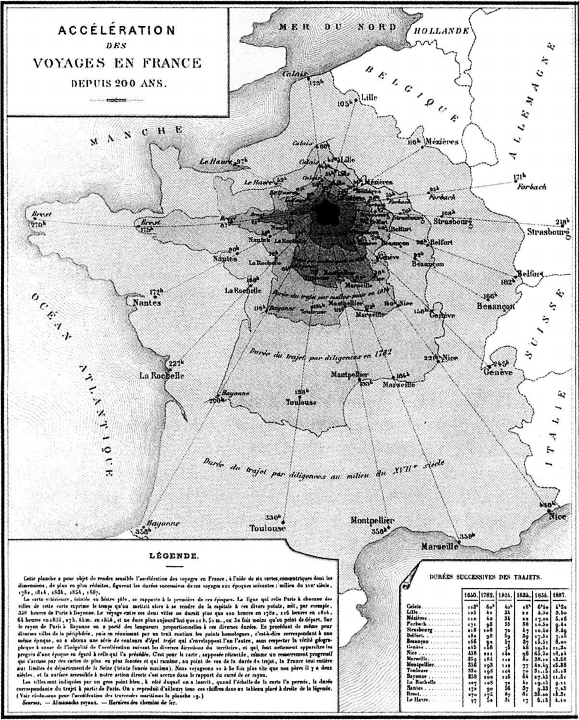
\includegraphics[scale=1, width=\columnwidth]{Vieille_Carte.png}
 \caption{\textit{Acceleration of travel times in metropolitan France during the past 200 years, dated from 1888} \cite{Cheysson} }
 \label{fig:sample}
\end{figure}

The visualization of traffic conditions and accessibility is, on the other hand, also a widely considered problem. It is actually an old issue, as shown in the following example: In the figure above one sees the changes of traveling time to Paris from other French cities, during a period of 200 years, which dates back to 130 years ago! For a discussion on this matter one can see \cite{schoedon2016interactive}.


Accessibility with respect to the railway mean of transportation is also an old issue, as there is a visualization of roughly the same epoch displaying travel times from Paris across the country. This can be found in \cite{vieillecartetrains}. A more interactive and recent visualization of travel times by the railway is for instance available in \cite{LeMonde1}. A comparison of accessibility within France territory with respect to both train, car and flight transportation is outlined in \cite{sauvant2002}.\\




There are several much-used techniques of visualization of travel times across a territory, most of them displaying a chart of the territory. One of these techniques consists in coloring the map according to travel times, and this is the approach we adopt here. Actually, our visualization is very close to the one displayed in Figure 2, as the authors noted after this work was performed. Another solution would be the \textit{isochrone maps}, which displays the zone a traveler may access form a given location and within a given amount of time. An alternative popular representation of accessibility is through \textit{anamorphic maps}, from which Figure 1 is an example: The map is deformed according to its travel time starting from a given city.  

\begin{figure}[!h]
 \centering % avoid the use of \begin{center}...\end{center} and use \centering instead (more compact)
 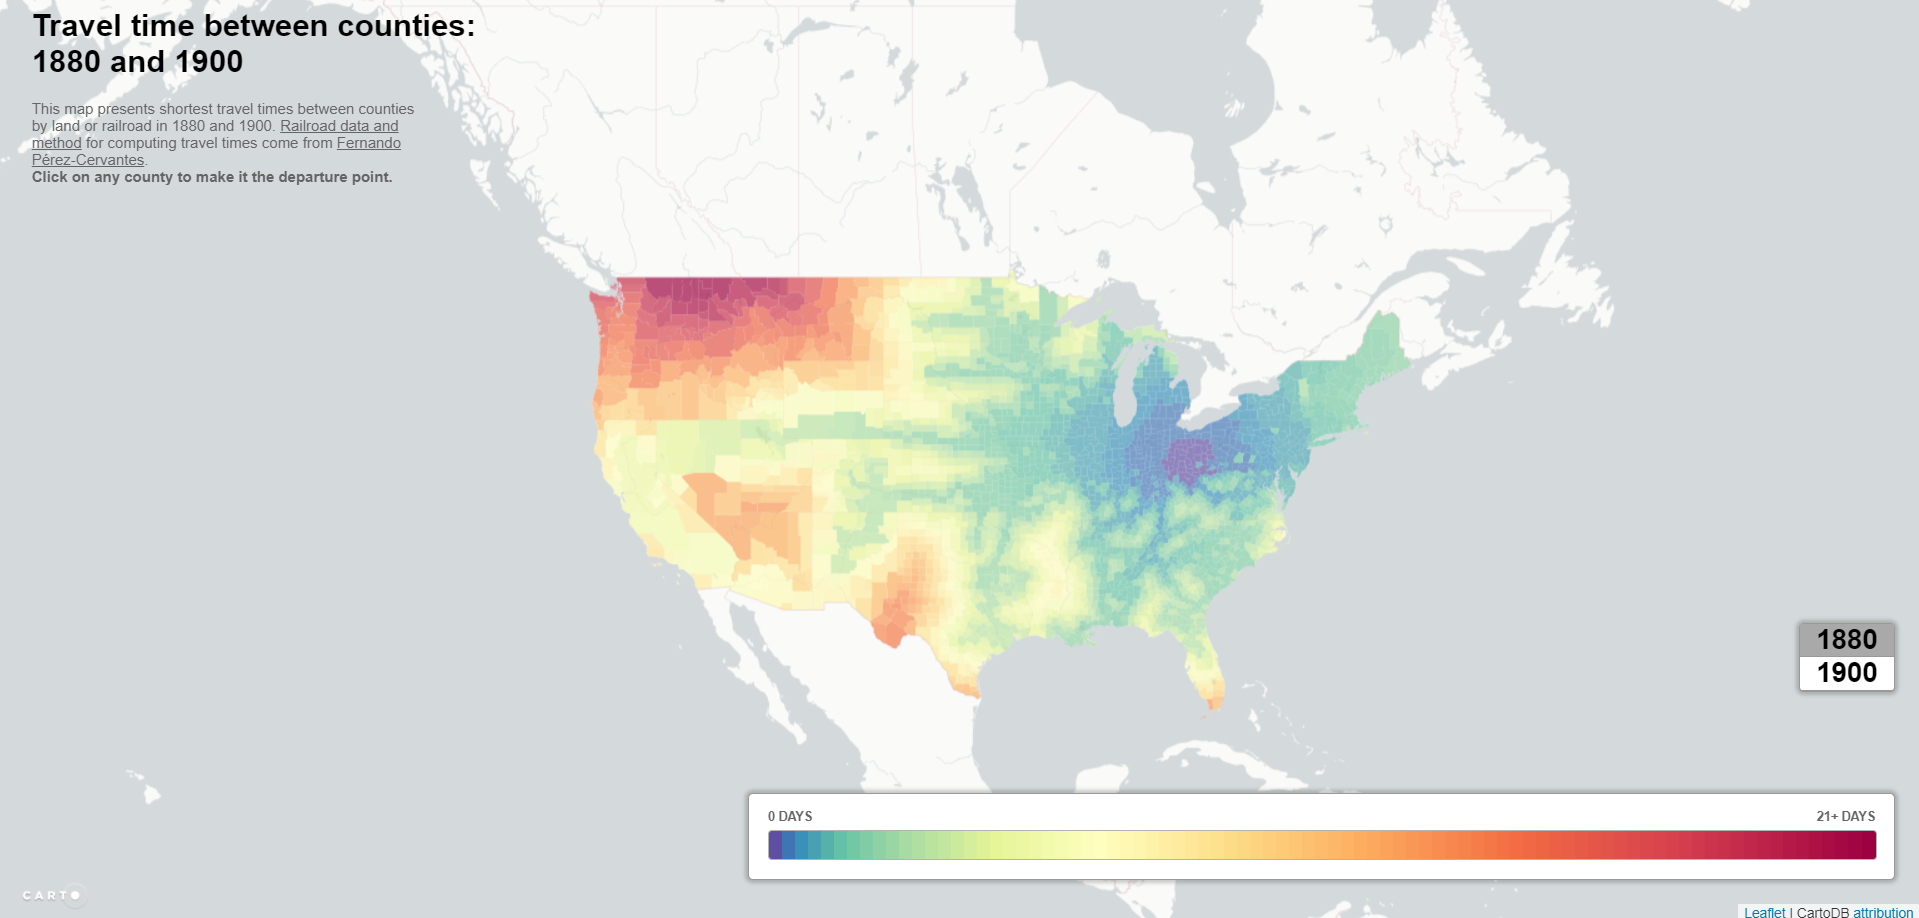
\includegraphics[scale=1, width=\columnwidth]{CarteInteractiveUSA.png}
 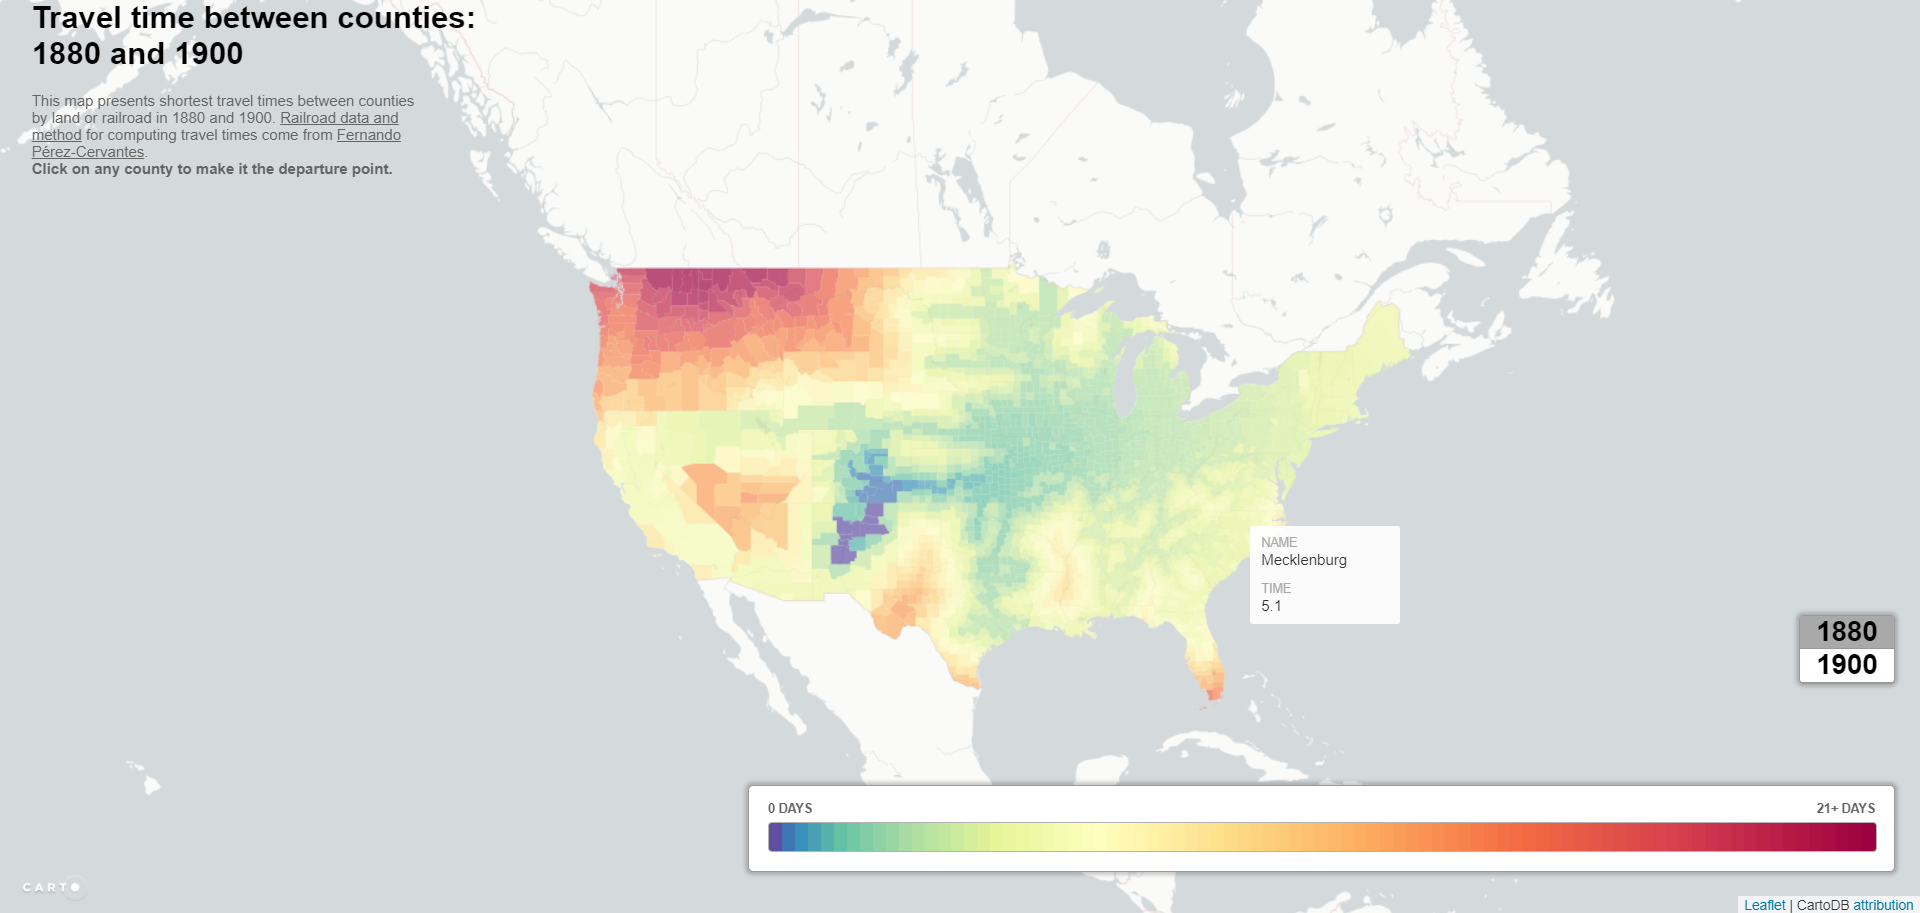
\includegraphics[scale=1, width=\columnwidth]{CarteInteractiveUSA_2.png}
 \caption{\textit{Interactive chart of travel times across the US as of the end of $19^{th}$ century } \cite{Moser} }
 \label{fig:sample}
\end{figure}


\section{Presentation of our visualization}

\vspace{0.1cm}

\subsection{Data acquisition}

\vspace{0.2cm}

The data of traveling time between two geographical points on the globe are extremely rich and can be obtained e.g. through the Google \textit{Distance Matrix} API \cite{APIGoogle},
by sending a request in form of a URL, in which information such as city of departure, city of arrival, means of transportation (automobile, bike or through the railway network when possible) and traveling date should be specified.  
  
%\vspace{0.2cm}


The number of journeys to be treated dramatically increases as more cities and dates are considered, and storing the entire amount of traveling times between all places that one can name all over the country is simply out of reach. Furthermore, as users of the free version of this service, we are only allowed to initiate requests with a very limited numbers of cities of departure and arrival (10 at a time), and it is thus necessary to parsimoniously select the cities to be considered. 


The considered cities must be of important size for better relevance, and must also be well distributed among the territory, while being of reasonable number. We chose to select the biggest city of each department of metropolitan France: This reduces the amount of cities to consider to about a hundred, which are from their very selection homogeneously distributed across the territory, and of maximal size under the two previous constraints. The use of the complete list of French agglomerations, as well as a short Python script, gives us the list of such cities.

Even if we are now reduced to about a hundred of cities it is still necessary to automatize the procedure of data acquisition. In order to build a matrix of travel times between any two of these cities, we have written a short Python program outputting the list of URL permitting, via Google's API, to collect these datas in groups of ten cities of departure and arrival (this is the limit Google puts on each request). There is a hundred of these URLs, for the same amount of resulting json files, a quantity that can be reduced to fifty five in assuming that the travel time from a point A to a point B is the same as from B to A. The result of these requests represents about five thousand data put into fifty five different json files, which is finally combined into a single json file thanks to a Python script.\\ 

At an advanced stage of the project we decided to add to this json file the amount of population living in the department of each city: This was easily accomplished using data collected by the INSEE institute of statistics on the year of 2014 \cite{INSEE} and using a Python script. The file resulting from these operations contains all the necessary data for our visualization. 




\begin{figure}[h]
 \centering % avoid the use of \begin{center}...\end{center} and use \centering instead (more compact)
 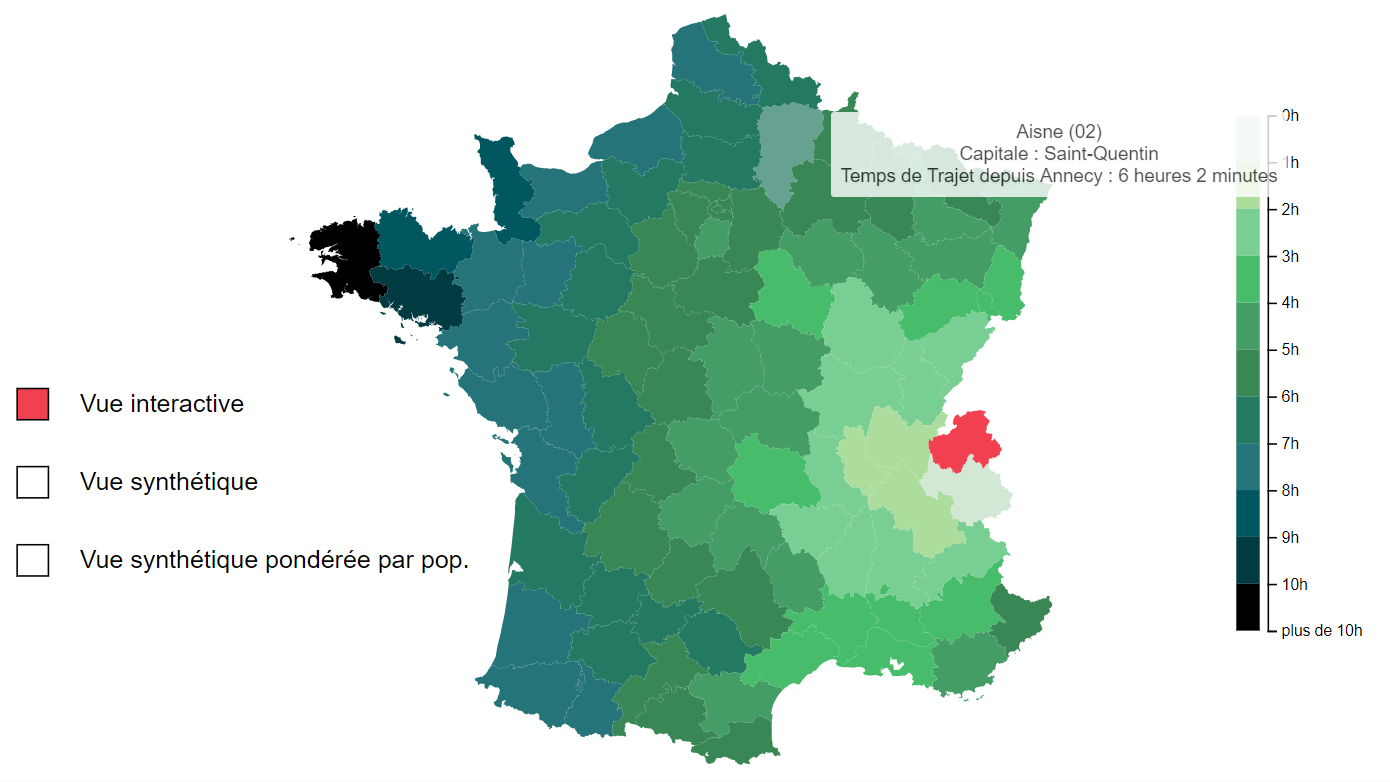
\includegraphics[scale=1, width=\columnwidth]{ImageProjet10_01.png}
 
 \vspace{0.4cm}
 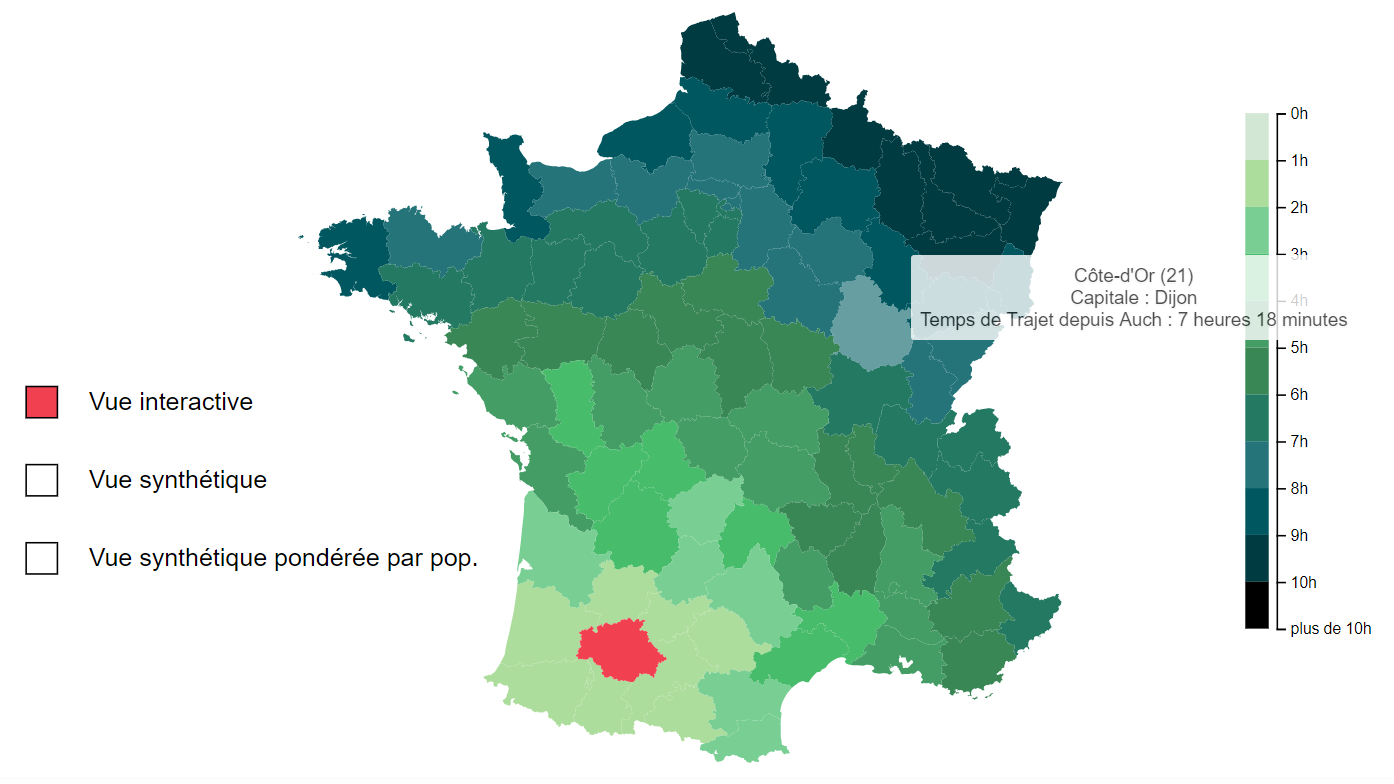
\includegraphics[scale=1, width=\columnwidth]{ImageProjet10_01_2.png}
 
  \vspace{0.4cm}
 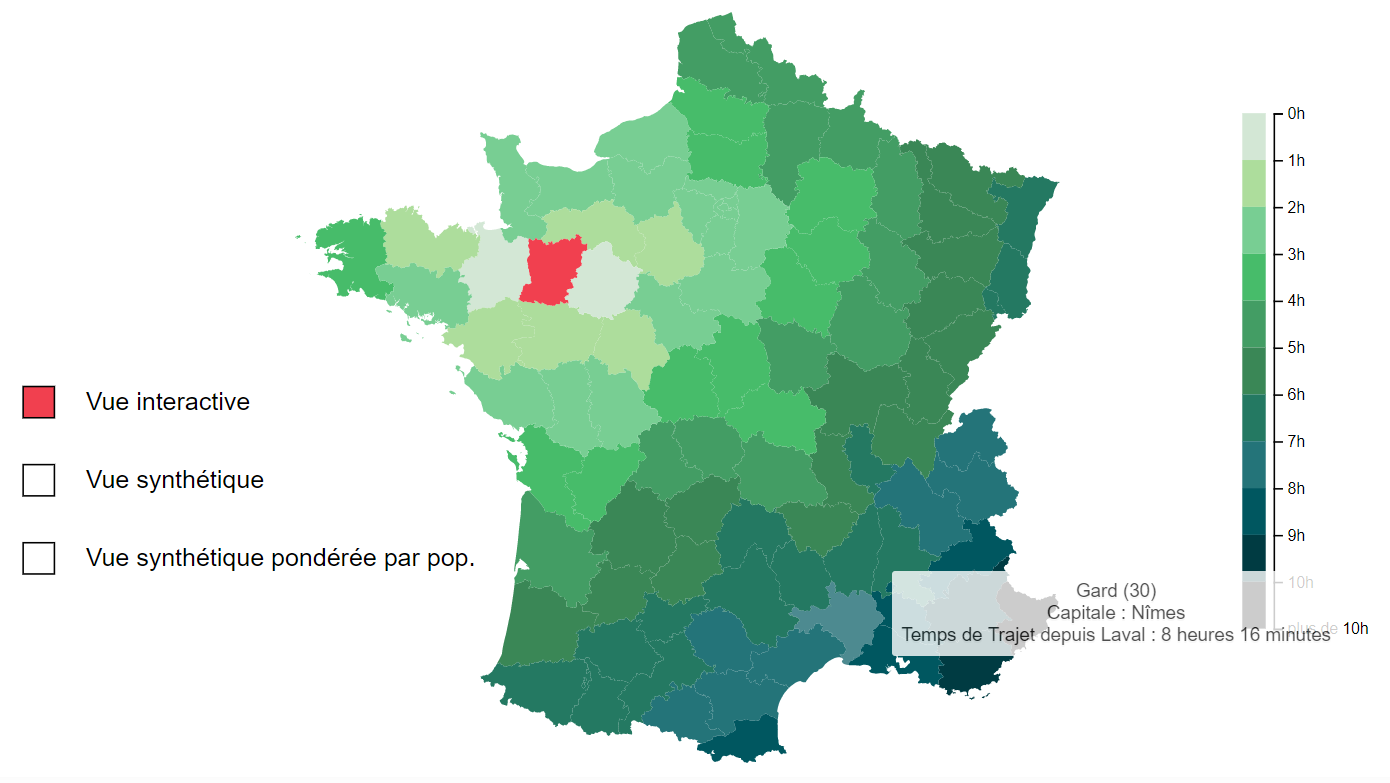
\includegraphics[scale=1, width=\columnwidth]{ImageProjet10_01_3.png}
 \caption{A sample of the interactive mode.}
 \label{fig:sample}
\end{figure}


\subsection{Implementation}

\vspace{0.2cm}


In this project, the javascript library d3.js will be our top priority as a visualizing tool, not only for its high compatibility with geodata, but also for the wide variety it offers in terms of graphical expressiveness of a map. As a result, among all technique details, our first concern will be to select the appropriate d3 template which could be as suitable as possible for our data type. Fortunately, there is a perfect existing 
 map of France that can be exploited here, standing in the form of a geojson file loadable in d3, and which shows in a very clean way metropolitan France together with its subdivision into departments. 
 
 


%\begin{figure}[!h]
 %\centering % avoid the use of \begin{center}...\end{center} and use \centering instead (more compact)
% 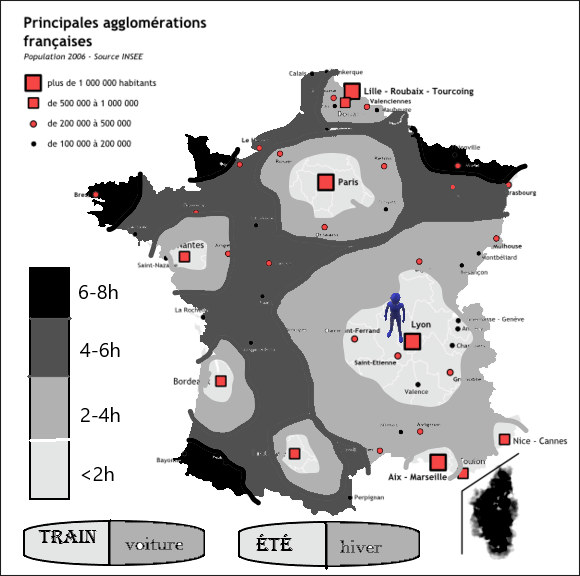
\includegraphics[scale=1, width=\columnwidth]{carte-france23.png}
% \caption{A visualization of traveling times towards the city of Lyon.}
% \label{fig:sample}
%\end{figure}

We would like to construct a continuous color map instead of isolated colorful cities, as thought at an early stage of the project. The advantages to use a colored map in our visualization are here very clear: one can not only rapidly grasp the accessibility of other places in France with respect to this city, but the comparison between traveling times and actual distances is also immediate. However, because it is impossible to include the entire amount of places of France in our calculation of distances, a solution of approximation need to be found for less populated cities and villages. This is where we use the mentioned subdivision into departments, by making the following approximation: we let the travel time between any two points on the map be the travel time between the capitals of their respective departments (where capital of a department means here its most populated city). In doing so, we extends the notion of travel time from our sample of cities to the whole map. We note that another natural subdivision of the territory could have been considered instead, for instance the one formed of the Voronoi cells one may construct about each of the cities considered. Another choice would have been to first consider a regular tiling of the territory, e.g. by squares or hexagons, and to color each tile accordingly (see the web blog \cite{smith} for a nice implementation of this idea). From the approximation we made, travel times now become features of the departments themselves rather than of their capitals.




\subsection{Visualization structure}




%The visualization of cities accessibility starts in the first place with a synthetic view: a topographic map of France, where "mountains" represent cities that are easier to access in general and valleys the ones who have a lower mean accessibility.  
  
The main part of the visualization takes the form of a national map, where a department is selected in advance, and from which travel times to other departments are displayed. In this visualization, whenever the user makes a click other a department then this one automatically becomes the department of origin in a new visualization. For this reason we call this mode the \textit{interactive mode}. Figure 3 below shows the travel times starting from three different choices of department of origin (pointed in red on the map). Lastly, representations of a network of main cities by means of graphs is treated in \cite{Gleyze}.


This visualization shows the amount of time that is necessary to travel from one given department to any other, and may also be seen as an interactive isochrone map, as it permits to see the area of territory that is reachable from any given department within a chosen time (for instance, the zone that is reachable from the Rhone department within five hours by car).

In each of the figures the cursor is pointed at another department, which is displayed on the map with slightly lower opacity, and from which we can see basic features as well as its travel time from the red department. Each color corresponds to an interval of time of one hour (one color between zero and one hour of travel time, another between one and two hours and so on), and coloration of the map goes with increasing intensity as the traveling time form the red department increases. 


For many of the departments, coloration shows a pattern of clear color  spreading vertically from the department, toward the top and bottom of the map. As clear color corresponds to short travel time, we conclude that the driving network is in general more efficient along vertical axes than along horizontal axes. A neat occurrence of this phenomenon is the comparison of the travel time between the farthest north/south departments and the farthest south-east/west departments: Although these two itineraries are roughly of the same distance at a bird's flight, the first is an approximately ten hours long trip whereas the second is more than thirteen hours long.\\


In addition to the interactive mode, the user is invited to select a \textit{synthesis mode} by means of a button put on the left-hand side of the chart. In this mode, interaction with the map is no longer possible, and the coloration displayed for any department corresponds to the travel time towards this department, after averaging out over the whole territory. A move on a department with the cursor makes it appear with slightly lower opacity, and shows the precise value of this averaged travel time, as presented in Figure 4 below.

With no surprise, territories located around the geographical center of the map are the more accessible ones in average. We also note the very good accessibility of the Parisian region, despite its non-centered location.







\begin{figure}[h]
 \centering % avoid the use of \begin{center}...\end{center} and use \centering instead (more compact)
 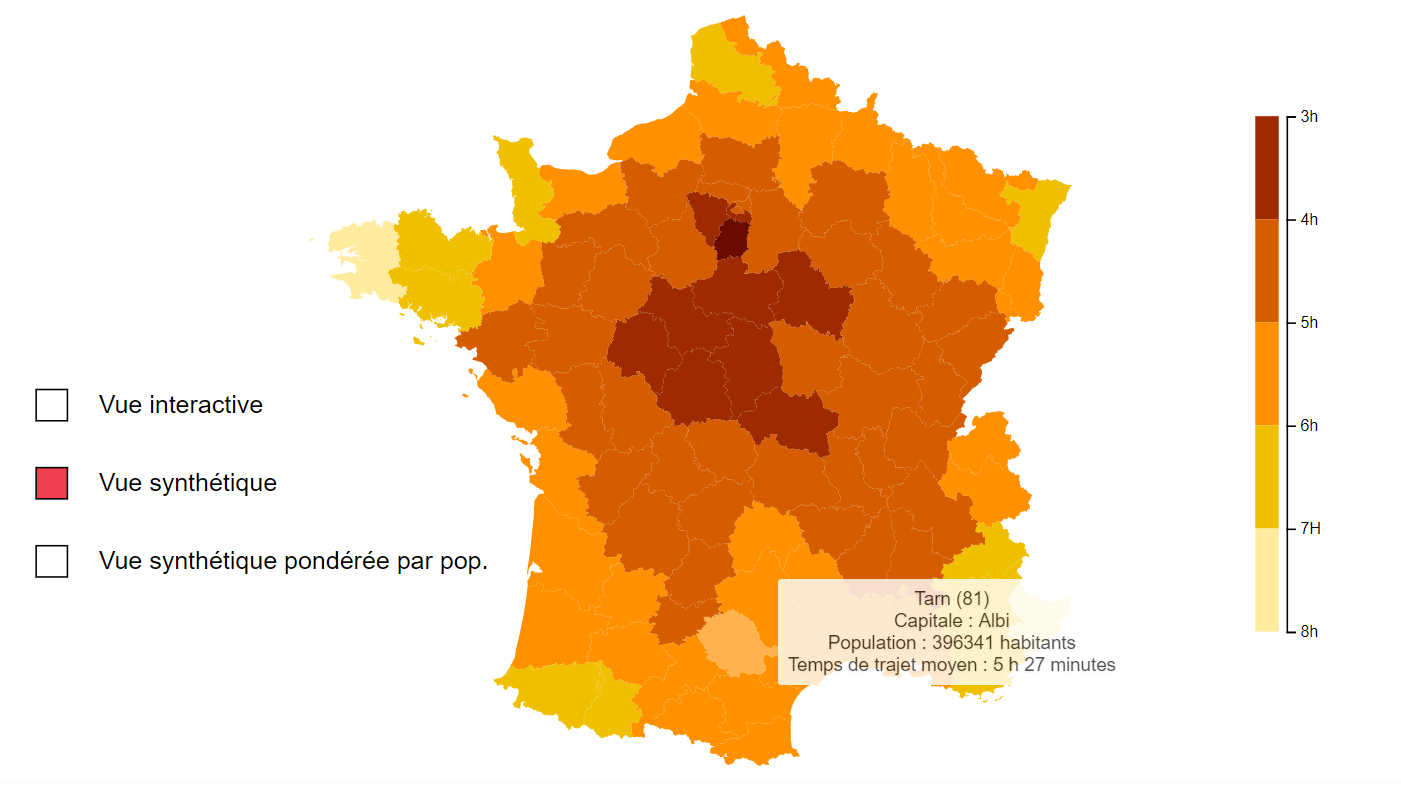
\includegraphics[scale=1, width=\columnwidth]{ImageProjet10_01_Bis.png}
 \caption{Synthesis mode, displaying travel times towards departments averaged out over the territory.}
 \label{fig:sample}
\end{figure}




Perhaps more interesting are the travel times towards departments with averaging taken over the \textit{population} rather than over the territory. Indeed, a department may appear well-accessible if it lies around the center of the map, but if only few people live at short travel time to it then it actually becomes an hardly accessible zone, since many people see it as a distant area. This observation led us to weight the travel time towards a department by the amount of population living in each department, yielding, for each department, travel time \textit{averaged over the population}. This view is displayed in a \textit{weighted synthesis mode}, which is pictured in Figure 5 below.

\begin{figure}[h]
 \centering % avoid the use of \begin{center}...\end{center} and use \centering instead (more compact)
 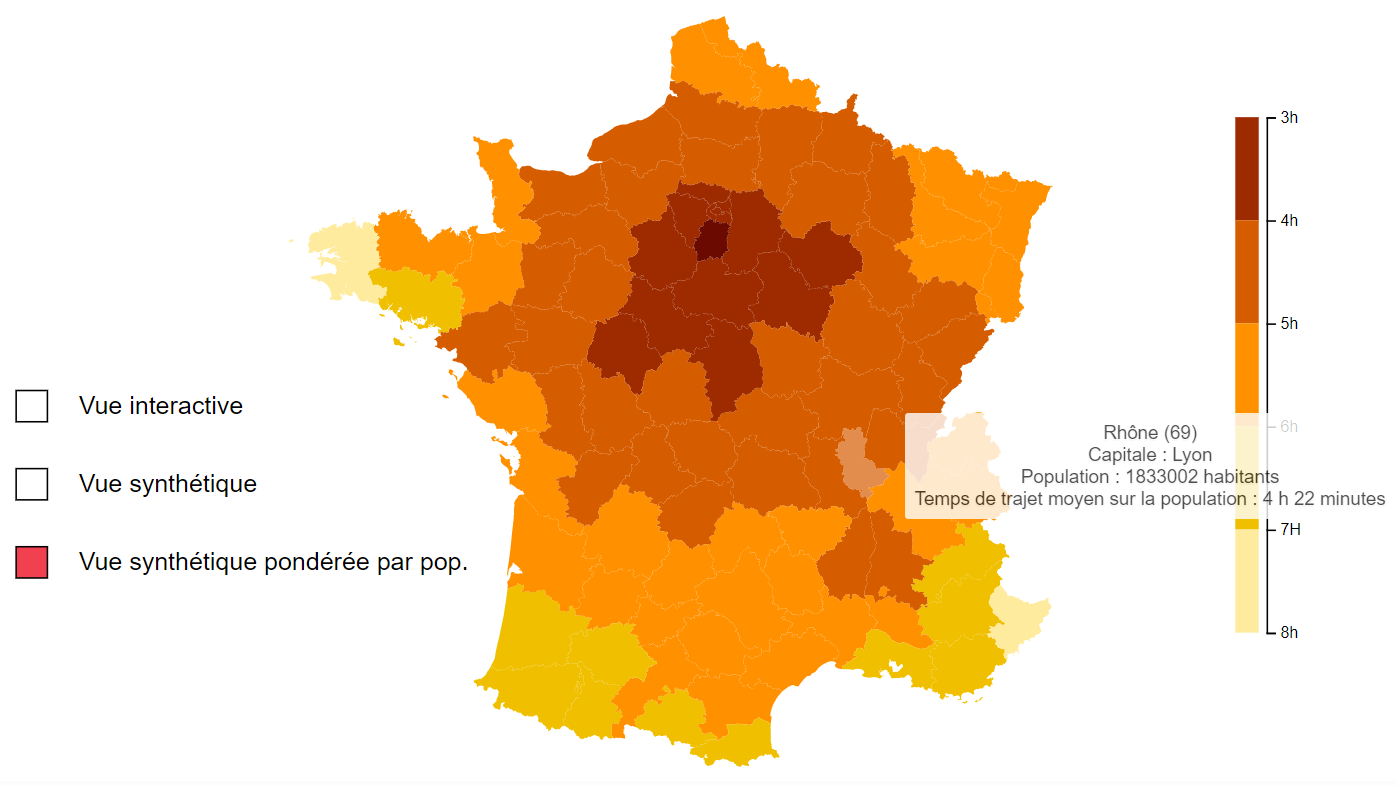
\includegraphics[scale=1, width=\columnwidth]{ImageProjet10_01_Ter.png}
 \caption{Weighted synthesis mode, displaying travel times towards departments averaged out over the population.}
 \label{fig:sample}
\end{figure}


In this view, we note a slight move of the most accessible zones from the geographical center towards Paris and its neighboring departments. This is not very surprising, since these regions are the most accessible ones for a lot of people. This also highlight the fact that much fewer people live in the south-western quarter of metropolitan France. 



\section{Conclusion and perspectives}

\vspace{0.2cm}

In this work we presented a visualization method of the accessibility of the different locations in metropolitan France, displaying how accessibility is distributed among the territory. We privileged a map structure which is simple, intuitive but also effective. A structure that could be further perfected in many ways. On the technical level, we may have made our visualization even more user-friendly by letting the selected department be connected to others using a arc, just like an airway course map with the traveling time in number in the middle over each arc. Moreover, we could eventually consider to animate them so that an arc joining faster the selected city represents a shorter traveling time. We may also focus a bit on the legend, and for each selected department display the amount of department of each color, thus providing a bar chart that supports the main visualization. 

On the level of the visualization's content, we wish we could have offered the user the ability to switch between railway and automobile as transportation mean and between summer and winter as the season the journey should take place in, for the reason that depending on the month of a year, the SNCF timetable and the road conditions of the highways may drastically vary. The time granularity may have been refined to get a better description of the impact of time on real-time accessibility of a city. Plus, we wished to give the user the possibility to select both of the transportation means, and in that case, the map had displayed two colors, each of them representing respectively train or car, indicating the quicker way to get to a place. Again, we find such representation with a colored map very attractive, in the way that
it could bring immediately the competitiveness of both transportation means to light.

 
 On a more speculative level, we may have raised whether well accessibility makes a city a significant destination, that is, whether it is accompanied with a lot of traffic towards it (compared to other destinations). We may go even further and compare accessibility of a city with its actual needs (in terms of importation/exportation of persons, materials and goods). This could have been compared with a further study of public transport users, that is, compare this map with the statistics on who travels: according to their age group, origin, motivation and so on. Another interesting perspective would have been to see whether we could eventually, in our calculation of general accessibility of a city, put weights on traveling times so that cities being far away are penalized. Indeed, one can naturally consider that accessibility of a city has a much more important meaning to its neighborhood than to some other city 300 km away. Of course a such modification would need finer mathematical treatments. Finally, one can also be concerned with the comparison of the socio-ecomonic impact of the city accessibility on a countrywide scale with that on a urbain-suburbain scale.



%% if specified like this the section will be committed in review mode
%\acknowledgments{
%The authors wish to thank A, B, and C. This work was supported in part %by
%a grant from XYZ.}

%\bibliographystyle{abbrv}
\bibliographystyle{plain}
%\bibliographystyle{abbrv-doi-narrow}
%\bibliographystyle{abbrv-doi-hyperref}
%\bibliographystyle{abbrv-doi-hyperref-narrow}

\bibliography{biblio}
\end{document}
